\message{ !name(<none>.tex)}
\message{ !name(<none>) !offset(27) }


\tableofcontents

\section{Each colom represent mean}
\label{sec:org0470bc1}
\begin{center}
\begin{tabular}{lll}
Column & Mean & remark\\
\hline
F (6) & ranking & \\
G (7) & Chinese origin data & \\
H (8) & Google translated data & \\
I (9) & Baidu Chinese sentiment analysis positive probability & base on Chinese origin data\\
J (10) & Baidu Chinese sentiment analysis confidence & base on Chinese origin data\\
K (11) & Baidu Chinese sentiment analysis Negative probability & base on Chinese origin data\\
L (12) & Baidu Chinese sentiment analysis the category & base on Chinese origin data\\
M (13) & Baidu English sentiment analysis positive probability & base on Google translated data\\
N (14) & Baidu English sentiment analysis confidence & base on Google translated data\\
O (15) & Baidu English sentiment analysis Negative probability & base on Google translated data\\
P (16) & Baidu English sentiment analysis the category & base on Google translated data\\
Q (17) & Google Chinese sentiment analysis score & base on Chinese origin data\\
R (18) & Google Chinese sentiment analysis manitude & base on Chinese origin data\\
S (19) & Google English sentiment analysis score & base on Google translated data\\
T (20) & Google English sentiment analysis manitude & base on Google translated data\\
U (21) & Yandex translated data & base on Chinese origin data\\
V (22) & Google English sentiment analysis score & base on Yandex translated data\\
W (23) & Google English sentiment analysis manitude & base on Yandex translated data\\
X (24) & Baidu translated data & \\
Y (25) & Google English sentiment analysis score & base on Baidu translated data\\
Z (26) & Google English sentiment analysis manitude & base on Baidu translated data\\
AA (27) & Baidu English sentiment analysis postitive probability & base on baidu translated data\\
AB (28) & Baidu English sentiment analysis confidence & base on baidu translated data\\
AC (29) & Baidu English sentiment analysis Negative probability & base on baidu translated data\\
AD (30) & Baidu English sentiment analysis the category & base on baidu translated data\\
AE (31) & Baidu postitive probability change to Google score standard & base on origin data Baidu sentiment analysis\\
AF (32) & Baidu postitive probability tranform to Google score standard & base on column M\\
\end{tabular}
\end{center}

\subsection{note}
\label{sec:orgbc09a97}
\begin{itemize}
\item Baidu sentiment analysis Category Note
\begin{itemize}
\item 2 mean to belong to the positive category, 1 mean to belong to the neutral category, and 0 mean to belong to the Negative category
\end{itemize}
\item Google sentiment analysis Note
\begin{itemize}
\item The score of a document's sentiment indicates the overall emotion of a document. The magnitude of a document's sentiment indicates how much emotional content is present within the document, and this value is often proportional to the length of the document.
\item A document with a neutral score (around 0.0) may indicate a low-emotion document, or may indicate mixed emotions, with both high positive and negative values which cancel each out. Generally, you can use magnitude values to disambiguate these cases, as truly neutral documents will have a low magnitude value, while mixed documents will have higher magnitude values.
\item "Clearly positive" and "clearly negative" sentiment varies for different use cases and customers. You might find differing results for your specific scenario. We recommend that you define a threshold that works for you, and then adjust the threshold after testing and verifying the results. For example, you may define a threshold of any score over 0.25 as clearly positive, and then modify the score threshold to 0.15 after reviewing your data and results and finding that scores from 0.15-0.25 should be considered positive as well.
\end{itemize}
\end{itemize}

\section{Baidu sentiment analysis}
\label{sec:org850032d}
\subsection{Baidu Chinese sentiment analysis}
\label{sec:org6947fd1}
\subsubsection{Baidu Chinese sentiment analysis positive probability histogram}
\label{sec:org749c9a0}
\begin{center}
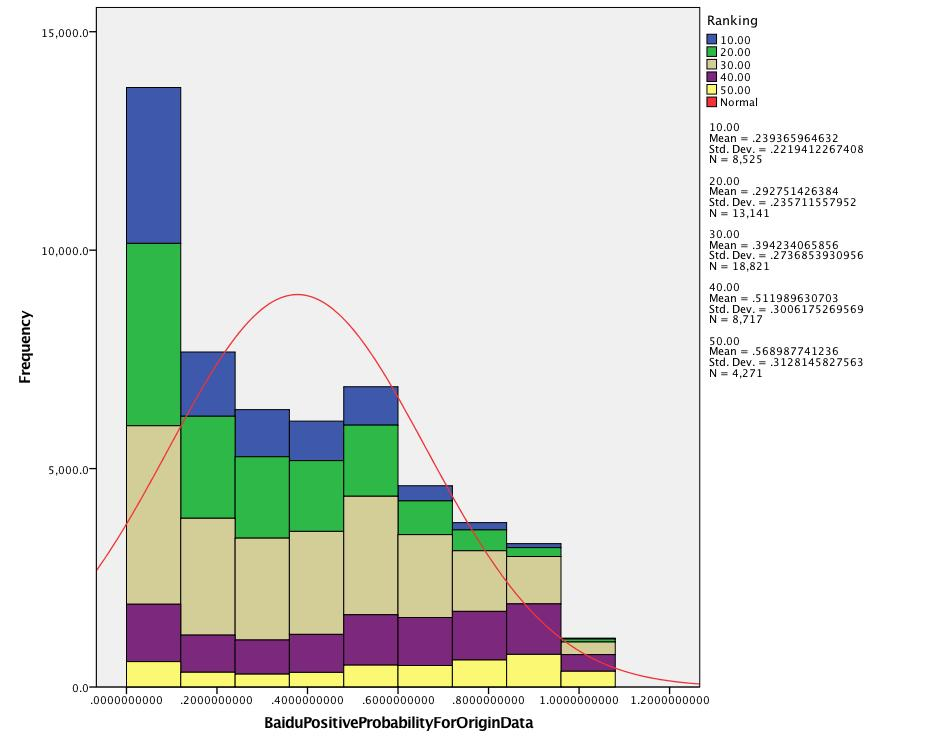
\includegraphics[width=.9\linewidth]{./img/BaiduPositiveProbababilityHistogramForOriginData.jpg}
\end{center}

\subsubsection{Baidu Chinese sentiment analysis postitive probability compare with different ranking(origin data)}
\label{sec:org2a96a0f}
\begin{center}
\begin{tabular}{lrrrrrr}
Ranking & Mean & Valid N & std.deviation & Total N & Minimum & Maximum\\
\hline
Ranking 10 & 0.239365965000 & 8525 & 0.2219412270000 & 8572 & 0.000106 & 1.000000\\
Ranking 20 & 0.292751426000 & 13141 & 0.2357115580000 & 13226 & 0.000162 & 1.000000\\
Ranking 30 & 0.394234 & 18821 & 0.273685 & 18974 & 0.000214 & 1.000000\\
Ranking 40 & 0.511990 & 8717 & 0.300618 & 8790 & 0.001050 & 1.000000\\
Ranking 50 & 0.568988 & 4271 & 0.312815 & 4307 & 0.000536 & 1.000000\\
\end{tabular}
\end{center}

\begin{center}
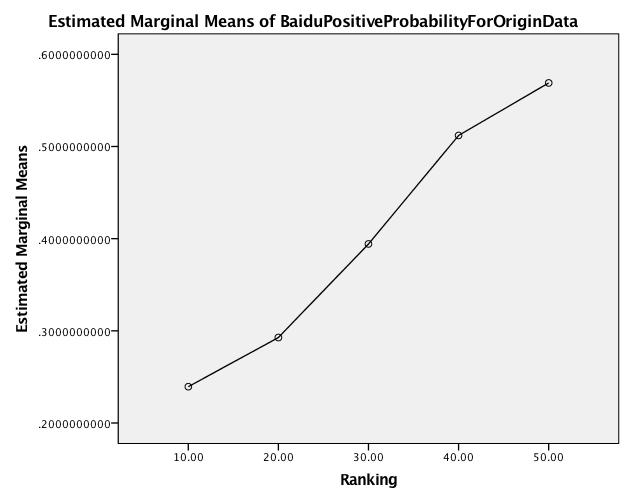
\includegraphics[width=.9\linewidth]{./img/MarginalMeansOfBaiduPositiveProbabilityForOriginData.jpg}
\end{center}

\begin{itemize}
\item Baidu Chinese sentiment analysis positive probability values are valid.
\end{itemize}

\subsubsection{Baidu Chinese sentiment analysis postitive probability tranform to Google Score standard compare with different ranking (origin data)}
\label{sec:org738019a}
\begin{center}
\begin{tabular}{lrrrlrrr}
Ranking & Mean & Valid N & std.deviation & Total N & Minimum & Maximum & Variance\\
\hline
Ranking 10 & -0.598875 & 8525 & 0.557595 &  & -0.999894 & 1.000000 & 0.310912\\
Ranking 20 & -0.488772 & 13141 & 0.617021 &  & -0.999838 & 1.000000 & 0.380715\\
Ranking 30 & -0.236524 & 18821 & 0.728420 &  & -0.999786 & 1.000000 & 0.530596\\
Ranking 40 & 0.054493 & 8717 & 0.773410 &  & -0.998950 & 1.000000 & 0.598164\\
Ranking 50 & 0.188983 & 4271 & 0.774245 &  & -0.999464 & 1.000000 & 0.599456\\
Total & -0.274854 & 53475 & 0.733884 &  & -0.999894 & 1.000000 & 0.538586\\
\end{tabular}
\end{center}

\begin{center}
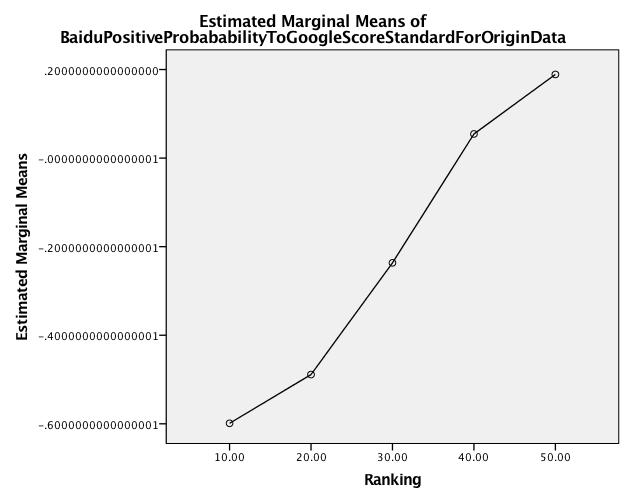
\includegraphics[width=.9\linewidth]{./img/MarginalMeansOfBaiduPositiveProbababilityToGoogleScoreStandardForOriginData.jpg}
\end{center}

\subsubsection{Baidu Chinese sentiment analysis category value compare with different ranking (origin data)}
\label{sec:org32005da}
\begin{center}
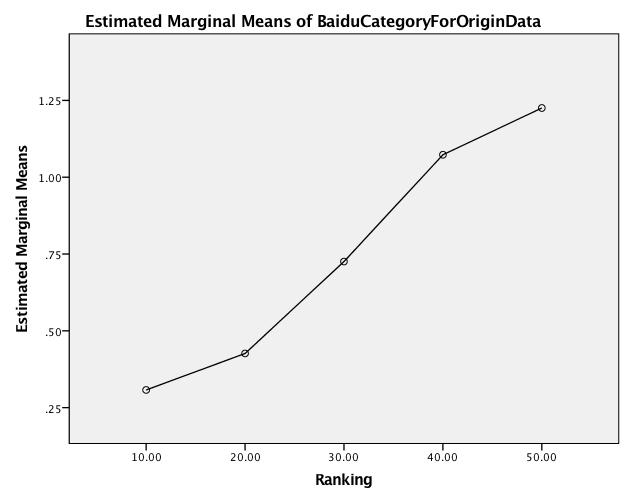
\includegraphics[width=.9\linewidth]{./img/MarginalMeansOfBaiduCategoryFroOriginData.jpg}
\end{center}

\begin{itemize}
\item Baidu Chinese sentiment analysis category values are valid.
\end{itemize}

\subsubsection{Chinese sentiment analysis Error Rate}
\label{sec:org6ed59fa}
\begin{center}
\begin{tabular}{lr}
Ranking & Error Rate\\
\hline
Ranking 10 & 0.0054829678\\
Ranking 20 & 0.0064267352\\
Ranking 30 & 0.0080636661\\
Ranking 40 & 0.0083048919\\
Ranking 50 & 0.0083584862\\
\end{tabular}
\end{center}

\begin{itemize}
\item Total Error Rate: 0.0073140396
\end{itemize}
\subsubsection{Baidu Chinese sentiment analysis Summary}
\label{sec:org1db4618}
\begin{itemize}
\item Baidu Chinese sentiment analysis positive probability values are valid.
\item Baidu Chinese sentiment analysis category values are valid.
\end{itemize}

\subsection{Baidu English sentiment analysis}
\label{sec:orgf18522b}
\subsubsection{Baidu English sentiment analysis postitive probability compare with different ranking (based on Google translated data)}
\label{sec:orgd634f3e}
\begin{center}
\begin{tabular}{lrrrlrrr}
Ranking & Mean & Valid N & Std.deviation & Total N & Minimum & Maximum & Variance\\
\hline
Ranking 10 & 0.517526 & 7968 & 0.134711 &  & 0.005045 & 1.000000 & 0.018147\\
Ranking 20 & 0.531020 & 12225 & 0.141214 &  & 0.037275 & 1.000000 & 0.019941\\
Ranking 30 & 0.540824 & 17457 & 0.137174 &  & 0.014443 & 1.000000 & 0.018817\\
Ranking 40 & 0.567782 & 8163 & 0.144971 &  & 0.051860 & 1.000000 & 0.021016\\
Ranking 50 & 0.589054 & 4006 & 0.150737 &  & 0.086614 & 1.000000 & 0.022722\\
\end{tabular}
\end{center}
\begin{center}
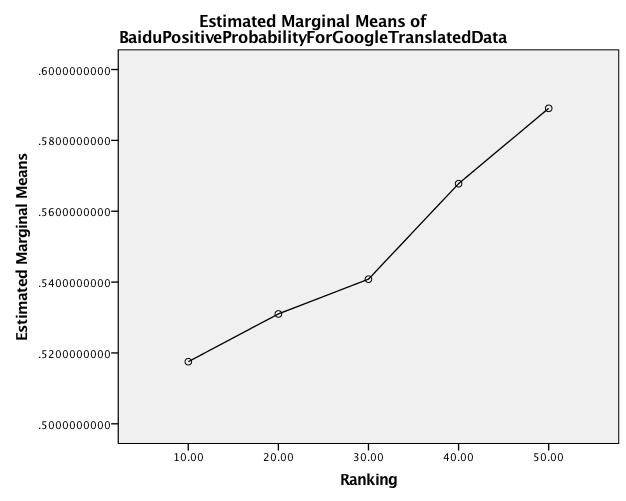
\includegraphics[width=.9\linewidth]{./img/MarginalMeansOfBaiduPositiveProbabilityForGoogleTranslatedData.jpg}
\end{center}

\begin{itemize}
\item Baidu English sentiment analysis positive probability values are valid.
\end{itemize}
\subsubsection{Baidu English sentiment analysis positive probability tranform to Google Score Standard (based on Google translated data)}
\label{sec:orge285725}
\begin{center}
\begin{tabular}{lrrrlrrr}
Ranking & Mean & Valid N & Std.deviation & Total N & Minimum & Maximum & Variance\\
\hline
Ranking 10 & 0.112029 & 7968 & 0.586700 &  & -0.994955 & 1.000000 & 0.344216\\
Ranking 20 & 0.150325 & 12225 & 0.587147 &  & -0.962725 & 1.000000 & 0.344742\\
Ranking 30 & 0.193858 & 17457 & 0.577416 &  & -0.985557 & 1.000000 & 0.333410\\
Ranking 40 & 0.276835 & 8163 & 0.564339 &  & -0.948140 & 1.000000 & 0.318479\\
Ranking 50 & 0.352409 & 4006 & 0.537822 &  & -0.913386 & 1.000000 & 0.289253\\
\end{tabular}
\end{center}

\begin{center}
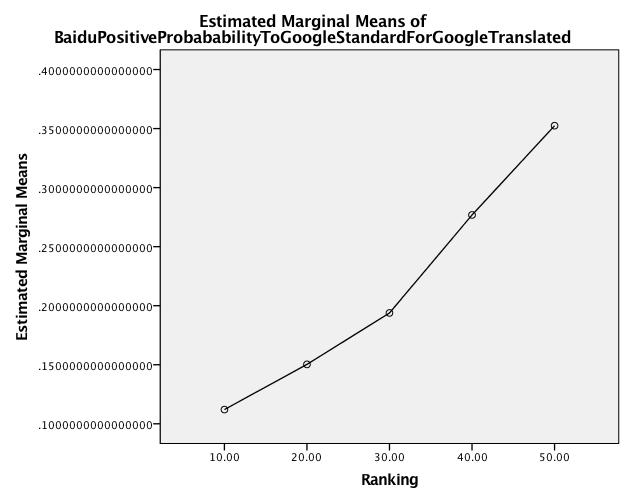
\includegraphics[width=.9\linewidth]{./img/MarginalMeansOfBaiduPositiveProbabilityToGoogleStandardFroGoogleTranslatedData.jpg}
\end{center}

\subsubsection{Baidu English sentiment analysis category values compare with different ranking (based on Google translated data)}
\label{sec:org4297533}
\begin{center}
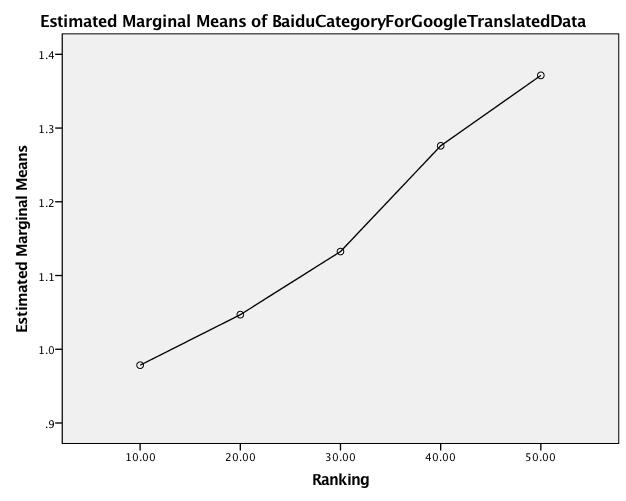
\includegraphics[width=.9\linewidth]{./img/MarginalMeansOfBaiduCategoryFroGoogleTranslatedData.jpg}
\end{center}
\begin{itemize}
\item Baidu English sentiment analysis category values are valid.
\end{itemize}

\subsection{Baidu Chinese sentiment analysis positive probability tranform to Google Score standard Method}
\label{sec:orgbecb070}
\begin{center}
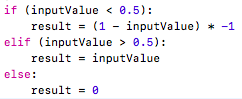
\includegraphics[width=.9\linewidth]{./img/baiduPositiveProbabilityTranformToGoogleScoreStandard.png}
\end{center}

\section{Google sentiment analysis}
\label{sec:org94c30eb}
\subsection{Google Chinese sentiment analysis}
\label{sec:org11ae8ea}
\subsubsection{Google Chinese sentiment analysis scores compare with different ranking (origin data)}
\label{sec:org70ba0e4}
\begin{center}
\begin{tabular}{lrrrrrr}
Ranking & Mean & Valid N & std.deviation & Total N & Minimum & Maximum\\
\hline
Ranking 10 & -0.238742 & 8567 & 0.445384 & 8572 & -0.900000 & 0.900000\\
Ranking 20 & -0.118380 & 13210 & 0.448064 & 13226 & -0.900000 & 0.900000\\
Ranking 30 & 0.117291 & 18940 & 0.462095 & 18974 & -0.900000 & 0.900000\\
Ranking 40 & 0.315915 & 8778 & 0.458128 & 8790 & -0.900000 & 0.900000\\
Ranking 50 & 0.361626 & 4305 & 0.441309 & 4307 & -0.900000 & 0.900000\\
\end{tabular}
\end{center}

\begin{center}
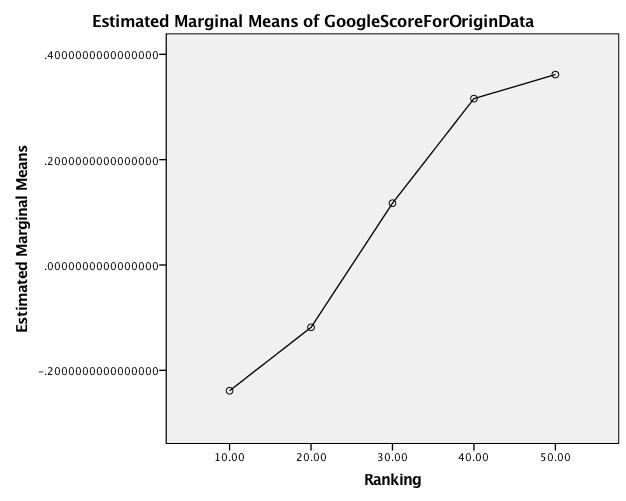
\includegraphics[width=.9\linewidth]{./img/MarginalMeansOfGoogleScoreForOriginData.jpg}
\end{center}

\begin{itemize}
\item Google Chinese sentiment analysis score values are valid.
\end{itemize}

\subsubsection{Google Chinese sentiment analysis Error Rate}
\label{sec:orgc10477d}
\begin{center}
\begin{tabular}{lr}
Ranking & Error Rate\\
\hline
Ranking 10 & 0.0005832944\\
Ranking 20 & 0.0012097384\\
Ranking 30 & 0.0017919258\\
Ranking 40 & 0.0013651877\\
Ranking 50 & 0.0004643603\\
\end{tabular}
\end{center}

\begin{itemize}
\item Total Error Rate: 0.0012808851
\end{itemize}

\subsection{Google English sentiment analysis}
\label{sec:org1f9c9de}
\subsubsection{Google English sentiment analysis score compare with different ranking (based on Google translated data)}
\label{sec:orga9d4397}
\begin{center}
\begin{tabular}{lrrrlrrr}
Ranking & Mean & Valid N & Std.deviation & Total N & Minimum & Maximum & Variance\\
\hline
Ranking 10 & -0.338431 & 8566 & 0.430581 &  & -0.900000 & 0.900000 & 0.185400\\
Ranking 20 & -0.244312 & 13204 & 0.437549 &  & -0.900000 & 0.900000 & 0.191449\\
Ranking 30 & -0.057978 & 18940 & 0.447353 &  & -0.900000 & 0.900000 & 0.200125\\
Ranking 40 & 0.147830 & 8777 & 0.455342 &  & -0.900000 & 0.900000 & 0.207336\\
Ranking 50 & 0.225000 & 4304 & 0.453471 &  & -0.900000 & 0.900000 & 0.205636\\
\end{tabular}
\end{center}
\begin{center}
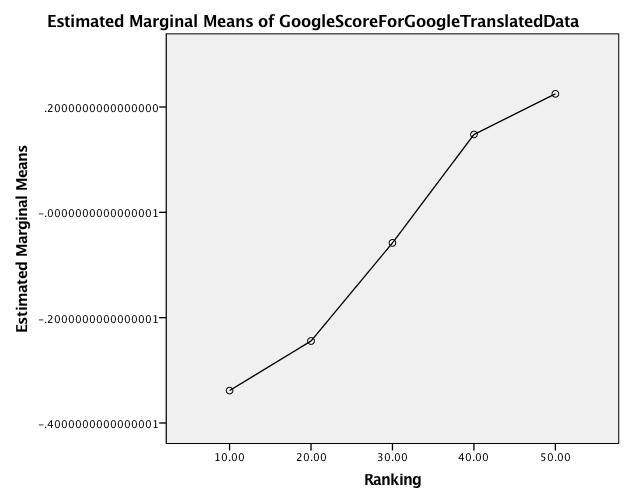
\includegraphics[width=.9\linewidth]{./img/MarginalMeansOfGoogleScoreFroGoogleTranslatedData.jpg}
\end{center}

\begin{itemize}
\item Google English sentiment analysis score values are valid based on Google translated data.
\end{itemize}

\subsubsection{Google English sentiment analysis score compare with different ranking (base on Yandex translated data)}
\label{sec:org946cd8b}
\begin{center}
\begin{tabular}{lrrrlrrr}
Ranking & Mean & Valid N & Std.deviation & Total N & Minimum & Maximum & Variance\\
\hline
Ranking 10 & -0.337873 & 8568 & 0.416416 &  & -0.900000 & 0.900000 & 0.173403\\
Ranking 20 & -0.233371 & 13221.000000 & 0.422133 &  & -0.900000 & 0.900000 & 0.178196\\
Ranking 30 & -0.055703 & 18972.000000 & 0.429758 &  & -0.900000 & 0.900000 & 0.184692\\
Ranking 40 & 0.138917 & 8788.000000 & 0.447876 &  & -0.900000 & 0.900000 & 0.200593\\
Ranking 50 & 0.208268 & 4306.000000 & 0.449598 &  & -0.900000 & 0.900000 & 0.202138\\
\end{tabular}
\end{center}

\begin{itemize}
\item Google English sentiment analysis score values are valid based on Yandex translated data.
\end{itemize}
\subsubsection{Google English sentiment analysis score compare with different ranking (base on Baidu translated data)}
\label{sec:org32a8312}
\begin{center}
\begin{tabular}{lrrrlrrr}
Ranking & Mean & Valid N & Std.deviation & Total N & Minimum & Maximum & Variance\\
\hline
Ranking 10 & -0.284984 & 8491.000000 & 0.416185 &  & -0.900000 & 0.900000 & 0.173210\\
Ranking 20 & -0.192064 & 13092.000000 & 0.417855 &  & -0.900000 & 0.900000 & 0.174603\\
Ranking 30 & -0.017125 & 18820.000000 & 0.429167 &  & -0.900000 & 0.900000 & 0.184185\\
Ranking 40 & 0.167667 & 8734.000000 & 0.432601 &  & -0.900000 & 0.900000 & 0.187144\\
Ranking 50 & 0.244657 & 4286.000000 & 0.430004 &  & -0.900000 & 0.900000 & 0.184904\\
\end{tabular}
\end{center}

\begin{itemize}
\item Google English sentiment analysis score values are valid based on Baidu translated data.
\end{itemize}

\subsubsection{Correlations Between Origin data, Google Translated data, Yandex Translated and Baidu Translated data (each element)}
\label{sec:org36da186}
\begin{center}
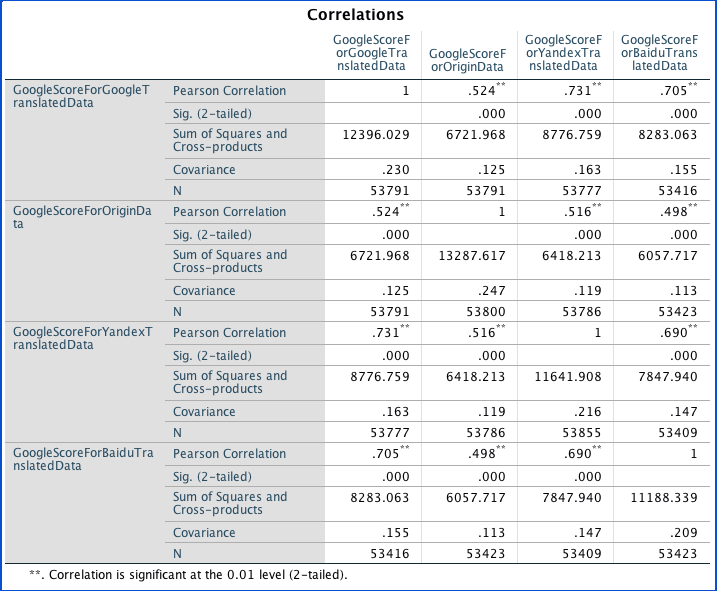
\includegraphics[width=.9\linewidth]{./img/correlationsBetweenOriginGoogleTranslatedYandexTranslatedBaiduTranslatedUsingGoogleSentiment.png}
\end{center}
\begin{itemize}
\item assumption Google English sentiment analysis tool and Google Chinese sentiment analysis tool are same
\begin{itemize}
\item Google translation sentence quality > Yandex translation sentence quality > baidu translation sentence quality
\item analysis same langeuage corrlations always bigger than cross langeuage corrlations
\end{itemize}
\end{itemize}

\subsubsection{Correlations between origin data Mean, Google translated data Mean, Yandex translated Mean and baidu translated data Mean}
\label{sec:org35a19ce}
\begin{center}
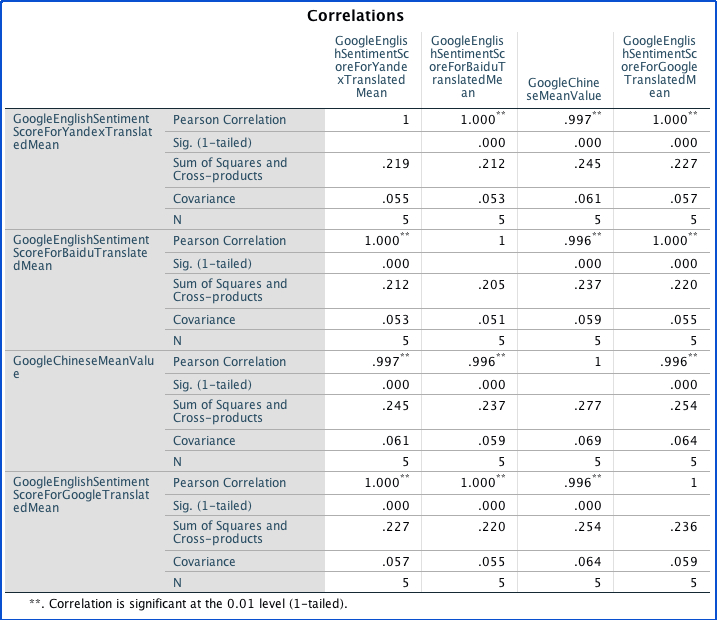
\includegraphics[width=.9\linewidth]{./img/correlationsBetweenOriginGoogleTranslatedYandexTranslatedBaiduTranslatedMeanUsingGoogleSentiment.png}
\end{center}
\begin{itemize}
\item translation sentence tools' quality have NOT significant impact sentiment analysis results
\item I guess translation key word quality more importance compare with sentence translation quality
\item Using sentiment analysis results compare different translation tools' quality are NOT reliable.
\end{itemize}

\section{Baidu sentiment analysis VS Google sentiment analysis}
\label{sec:org70a7cb7}
\subsection{Baidu Chinese sentiment analysis VS Google Chinese sentiment analysis}
\label{sec:orgd824a64}
\subsubsection{Mean Value Correlation}
\label{sec:org274133c}
\begin{itemize}
\item Pearson Correlation 0.991
\item sig. 0.001
\item N 5
\item Conclusion
Baidu Chinese sentiment analysis and Google Chinese sentiment analysis have higher liner relationship.
\end{itemize}

\subsubsection{Error Rate}
\label{sec:org39b131e}
\begin{itemize}
\item Baidu Chinese sentiment analysis Total Error Rate = 0.0073140396
\item Google Chinese sentiment analysis Total Error Rate = 0.0012808851
\item conclusion
\begin{itemize}
\item Baidu sentiment analysis error rate high than Google sentiment analysis error rate
\end{itemize}
\end{itemize}

\subsubsection{Tendency}
\label{sec:orgf129605}
\begin{itemize}
\item chinese sentiment analysis results given by both Baidu and Google are valid because when the ranking group ID increases from 11 to 50, the sentiment analysis score also strictly increases accordingly.
\end{itemize}

\subsection{Baidu English sentiment analysis VS Google English sentiment analysis}
\label{sec:org6a6efbc}
\subsubsection{Mean Value Correlation (based on Google translation)}
\label{sec:orgd406589}
\begin{itemize}
\item Pearson Correlation 0.978
\item sig. 0.004
\item N 5
\item Conclusion
Baidu English sentiment analysis and Google English sentiment analysis have higher liner relationship.
\end{itemize}
\subsubsection{Tendency}
\label{sec:org4fa1f32}
\begin{itemize}
\item English sentiment analysis results given by both Baidu and Google are valid because when the ranking group ID increases from 11 to 50, the sentiment analysis score also strictly increases accordingly.
\end{itemize}
\end{document}
\message{ !name(<none>.tex) !offset(-372) }
